%We present the experimental results of \sys's performance. We start with describing the hardware environment (Section~\ref{sec:results_hardware}) followed by the software environment (Section~\ref{sec:results_software}) and we concluded by the evaluation results (Section~\ref{sec:results_evaluation}).

\subsection{Hardware Suite Description}
\label{sec:results_hardware}

In all experiments we used the following computing hardware: WISP\,5.1~\cite{wisp5,wisp} build around MSP430FR5969~\cite{wolverine} 64\,kB FRAM microcontroller. WISP\,5.1 has been re-programmed during experiments using TI's Flash Emulation Tool (FET)~\cite{fet} with TI Code Composer Studio version 7. FET was also used as a power supply in non-intermittent power experiments. Energy consumption measurements provided in eariler sections were done with Carnegie Mellon's EDB~\cite{edb}. In experiments involving wireless power, the WISP was powered through an RFID reader (Impinj R1000 with firmware version 3.2.4.240~\cite{r1000_data_sheet}) connected to the Liard RFMAX S9028PCRJ 8\,dBic~\cite{atlas2015}. The RFID reader is controlled by a PC running Ubuntu 10.4 executing an open source Python-based \emph{sllurp} library~\cite{sllrp_github}. Transmitted power of the RFID reader was 30\,dBm at 915\,MHz center frequency. For distance-controlled experiments, the WISP was positioned at varying length hollow paper tubes placed directly on a flat lying antenna. Code execution times were measured using Salea~\cite{saleae} logic analyzer.

We also used an alternative setup where the MSP-TS430RGZ48C launchpad was used for continuous power experiments. We used internal timer for measuring run time. For harvested energy, we used the ThingMagic Astra-EX RFID antenna set at 30\,dBm transmission power. We used EDB~\cite{edb} to measure run time. Applications were cross-compiled using GCC and Clang, so that we can use LLVM for \sys compiler. Version 3.8.0 was used for both Clang and LLVM.

\subsection{Software Suite Description}
\label{sec:results_software}

We compare \sys against state-of-the-art task-based runtime Chain~\cite{chain}. We are not comparing \sys against DINO~\cite{dino} or Mementos~\cite{mementos} (Refer to Section~\ref{sec:background_consistency}), as (i) Chain is the only modular execution model available to which we can compare \sys, and (ii) Chain proved already its superiority over sequential model counterparts (i.e. DINO and Mementos)\footnote{We need to note that although another very relevant task-based runtime has been recently presented and referenced many times throughout this paper---Alpaca~\cite{alpaca} (written by the same group as Chain)---except the recently accepted manuscript we did not have the access to Alpaca's code during the preparation of this paper. Therefore Alpaca was excluded from the evaluation.}.

The applications that were used in the evaluation are: (i) \textbf{bc}: counts bits in byte pseudo-random string using varying algorithms. Each result is compared for correctness; (ii) \textbf{cem}: emulates an embedded temperature sensing engine: measurements are randomly generated and are compressed using a LZW algorithm for  fixed entry dictionary and fixed byte block; (iii) \textbf{cuckoo}: implements Cuckoo filter---the program first stores a sequence of pseudo-random numbers, then queries the filter to recover it; (iv) \textbf{rsa}: encrypts predefined string with a predefined key; (v) \textbf{ar} performs nearest neighbour classification using randomly generated sequence of three-axes accelerometer data. This set of benchmarks is the same as used in~\cite{chain,alpaca}. In addition to Chain benchmarks new applications were implemented: (vi) \textbf{dft}: discreet Fourier transform, (vii) \textbf{dd}: Huffman-based data decompression, and (viii) \textbf{sort}: selection sort algorithm. All applications are compared in Table~\ref{table:benchmark_list} in terms of source lines of code against Chain.

%\begin{table}[t]
%	\centering
%	\footnotesize
%	\begin{tabular}{|c|c|c|}
%		\hline
%		Application & SLOC (\sys) & SLOC (Chain~\cite{chain})\\
%		\hline\hline
%		{bc} & 351 & 588 \\ %59\%
%		{cem} & 388 & 721 \\ %53\%
%		{cuckoo} & 483 & 762 \\ %63\%
%		{rsa} & 887 & 1233 \\ %71\%
%		{ar} & 483 & 762 \\ %63\%
%		{dft} & {} & {} \\ %Two resolutions: 4 and 8 Bytes
%		{dd} & {} & {} \\ %Data decompression size: 100 bytes
%		{sort} & {} & {} \\
%		\hline
%	\end{tabular}
%\caption{List of benchmark programs used in \sys evaluation; SLOC: source lines of code.}
%\label{table:benchmark_list}
%\end{table}

\subsection{\sys Evaluation Results}
\label{sec:results_evaluation}

\subsubsection{\sys Compiler Performance}
\label{sec:results_compiler}

\begin{table}[t]
	\centering
	\footnotesize
        \renewcommand{\tabcolsep}{1pt}
	\begin{tabular}{|l|cc|cc|cc|cc|c|}
		\hline\hline
		{} & \multicolumn{2}{l|}{{\bf Prot. bytes}} & \multicolumn{2}{c|}{{\bf \# Tasks}} & \multicolumn{2}{c|}{{\bf \# Prot. acc.}} & \multicolumn{2}{c|}{\bf SLOC} & {\bf Comp.} \\
		App & Man. & Comp. & Man. & Comp. & Man. & Comp. & \multicolumn{1}{l}{\sys} & \multicolumn{1}{r|}{Chain~\cite{chain}} & {\bf time} \\
		\hline
		bc & 22 & 22 & 10 & 15 & 81 & 93 & 351 &588 & 3\\
		cem & 3492 & 3242 & 12 & 9 & 92 & 123 & 388 &721 & 2\\
		cuckoo & 282 & 288 & 15 & 6 & 90 & 76 & 483 &762 & 6\\
		rsa & 332 & 250 & 20 & 27 & 130 & 296 & 887 &1233 & 86\\
		ar & 166 & 218 & 11 & 6 & 112 & 333 & 483 &762 & 34\\
		sort & 104 & 104 & 4 & 2 & 70 & 23 & 180 & 287 & $<$1\\
		dft* & - & - & - & - & - & - & 222 & 293 & -\\
		dd &  &  &  &  &  &  &  & 287 &  \\
		\hline
	\end{tabular}
	\caption{Comparison between compiler-generated \sys code (Comp.) and hand-written \sys code (Hand). *DFT does not compile with Clang\todo{incomplete table}{Responsible:Kiwan}}
\label{table:compiler_result}
\end{table}

We start with evaluating the efficiency of the \sys compiler Table~\ref{table:compiler_result} shows the difference in the number of protected variables (PVAR), number of tasks, and number of inserted paging macro ({\tt RVAR} and {\tt WVAR}) in the code between (i) hand-written \sys and (ii) compiler-generated \sys code. On average, compiler-generated code is only worse by 0.3\% in the number of protected variables. Regarding the number of tasks, compiler-generated code is better by roughly 16\%. The results indicate that \sys compiler is selecting boundaries better than the programmer doing it manually. However, the \sys compiler should insert paging code conservatively when it {\em may} access protected variables, due to limitation of pointer aliasing. Thus, it results in the \sys compiler introducing 48\% more paging code than programmer-written code (the results on run time for various \sys code versions is provided in Section~\ref{sec:result_compiler_time}). The performance is worse than programmer-written \sys code in overall, meaning the programmer should structure the code manually if the performance is critical; otherwise the compiler can be used to simplify the programmability. 

Additionally, we evaluated the compile time for automatic task generation per application\footnote{We could not compile the DFT application since LLVM inserts mathematical built-in functions (i.e. \texttt{\_\_muldf3}, \texttt{\_\_floatsidf}, \texttt{\_\_adddf3}) whose implementation were not provided by the LLVM MSP430 back-end.}. We compiled the apps on a 4-core virtual machine with 1\,GB memory with Arch Linux, running on Intel Core i5-6200U (2.30\,GHz) processor. The result are given in Table~\ref{table:compiler_result}. We used the {\tt time} linux command to measure the rough time. Most of the compile time was due to pointer aliasing, when calculating possible live ranges of variables. Apps such as RSA whose code size is large and uses a lot of variables, need longer compilation time due to a larger search space for pointer aliasing.

%\begin{table}[t]
%	\centering
%	\footnotesize
%	\begin{tabular}{|c|c|c|c|c|c|}
%		\hline
%		bc & cem & cuckoo & rsa & ar & sort \\
%		\hline\hline
%		3 & 2 & 6 & 86 & 34 & < 1 \\
%		\hline
%	\end{tabular}
%	\caption{\sys compile time per application (seconds).}
%\label{table:compile_time}
%\end{table}
%
%\subsubsection{Task Coalescing Performance}
%\label{sec:results_coalescing}

%List of figures: 
%\begin{itemize}
%	\item Fig. 1: Viper only/per app/fixed power/(hand/complier)/no coalescing/clang [Resuls are ready by Kiwan]
%	\item Fig. 2: Viper only/per app/per distance (fixed/20/40/60)/(hand/complier)/coalescing [Resuls are ready by Kiwan]
%	\item Fig. 3a: (Viper Coalescing/Chain)/per app/per distance (fixed/20/40/60)/complier/clang [Resuls are ready by Kiwan]
%	\item Fig. 3b: (Viper Coalescing/Chain)/per app/per distance (fixed/20/40/60)/complier/gcc [Resuls are not ready: Kiwan needs to make them]
%	\item Fig. 4: exactly as Fig 12 in the paper (4 apps only)
%	\item Fig. 5: average virtual task size/gcc/fixed distance/per app 
%\end{itemize}

\subsubsection{\sys Runtime Performance}
\label{sec:result_coalescing}

\begin{figure}
	\centering
	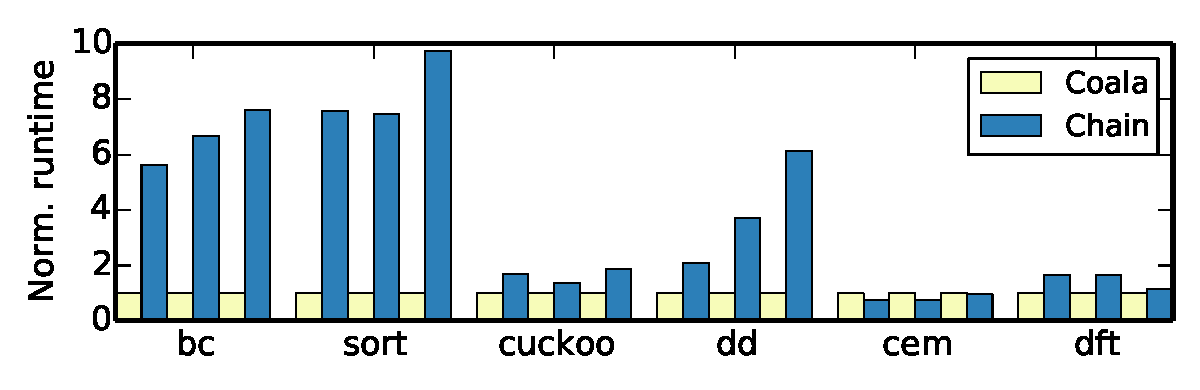
\includegraphics[width=\columnwidth]{figures/coala_chain}
	\caption{Performance of \sys's fixed power and at multiple WISP to RFID reader antenna distances, \{20, 40, 60\}\,cm, compared against Chain.}
	\label{fig:coalescing}
\end{figure}

Experimental evaluation of task coalescing mechanism under intermittent power of \sys is given in Figure~\ref{fig:coalescing}. For each application we measured execution time (with and without task coalescing) at \{20, 40, 60\}\,cm distance between RFID antenna and WISP and when WISP was powered directly from FET. Each measurement was repeated x times per each distance/application. From the result we clearly see an enormous benefit of coalescing, especially at large WISP to RFID reader antenna distance ($\approx$56\% for cem, 100\% for sort and $\approx$400\% for bc). At each distance, \sys coalescing mechanism provided faster execution times compared to the non-coalescing case. \todo{Discuss different shapes per app}{Amjad}

%\begin{figure}
%	\centering
%	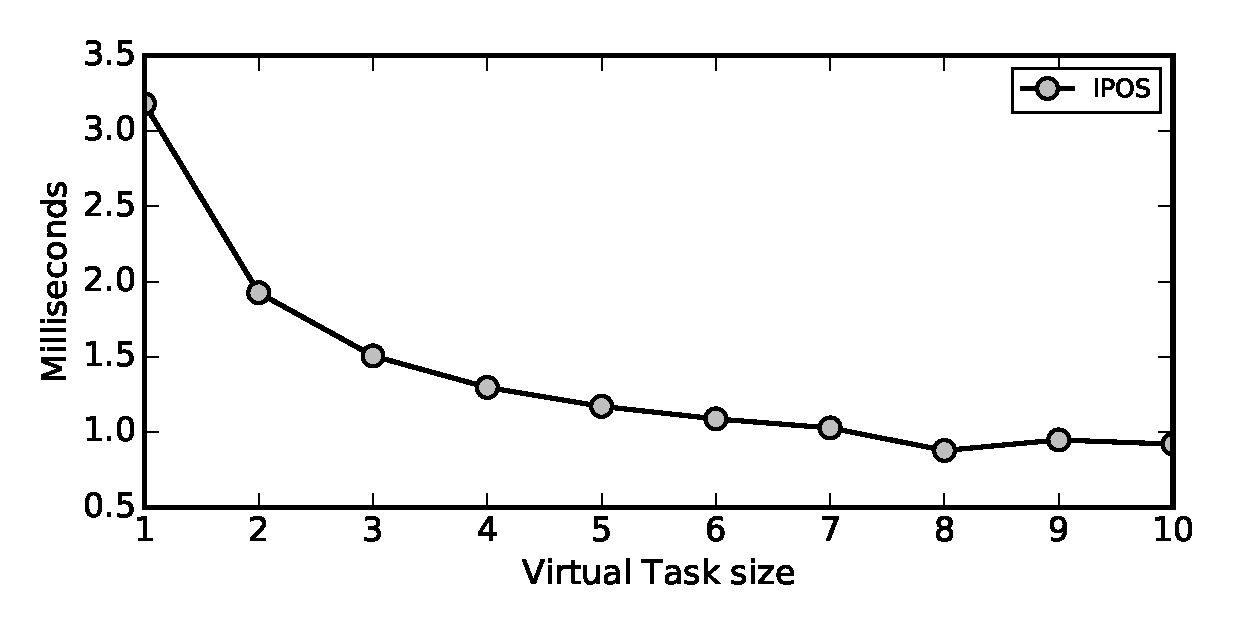
\includegraphics[width=\columnwidth]{figures/virtualTaskSize.eps}
%	\caption{Execution time of a dummy application containing twelve empty tasks as a function of coalescing factor. We observe three times improvement from coalescing until four virtual tasks, while we observe a diminishing return from task coalescing beyond four. \todo{Improve the figure: make it narrower, larger font, remove legend, do not capitalize "Task" in X axis, add Y axis label (Execution time (ms))}{Amjad}}
%	\label{fig:virtualTaskSize}
%\end{figure}

%The question remains: does coalescing all program's tasks into a singe virtual task (as the energy becomes fully available, i.e. from energy harvesting to continuous power environment) is the best one? To answer this question we have implemented a simple program composed of $x$ empty tasks. We execute the same program by increasing coalescing factor by one while the device on which the program was executed was running on a stable power supply (refer to Section~\ref{sec:methodology_evaluation} for details). The result is presented in Figure~\ref{fig:virtualTaskSize}. We observe a significant increase in execution time as task are coalescent from one to four (three times execution time improvement). However, as the coalescing increases beyond four, we observe diminishing returns from coalescing in terms of execution time. \todo{Decide whether to place this figure in Evaluation section or leave it here}{Przemek}

\subsubsection{\sys Compiler Overhead}
\label{sec:result_compiler_time}

\begin{figure}
	\centering
	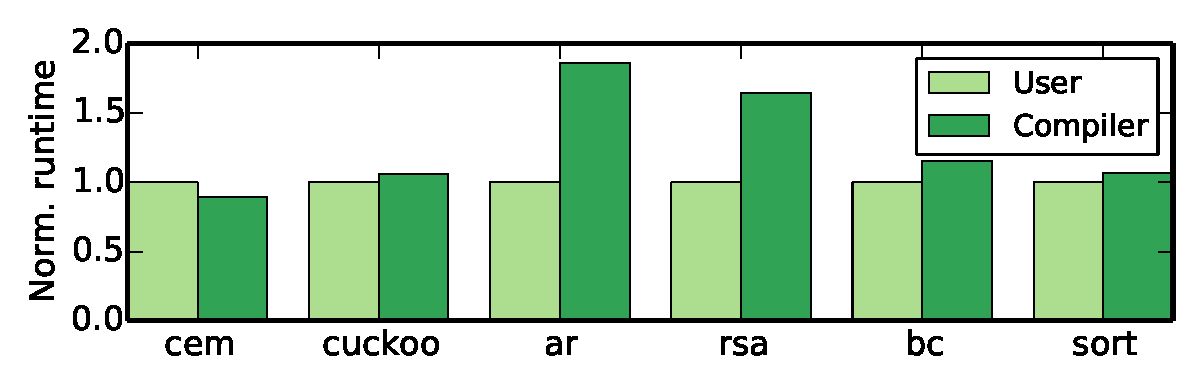
\includegraphics[width=\columnwidth]{figures/comp_user}
	\caption{\sys compiler overhead measured per application.}
	\label{fig:comp_user}
\end{figure}

Result is provided in Figure~\ref{fig:comp_user}.

\subsubsection{\sys Coalescing Performance}
\label{sec:result_compiler_time}

\begin{figure}
	\centering
	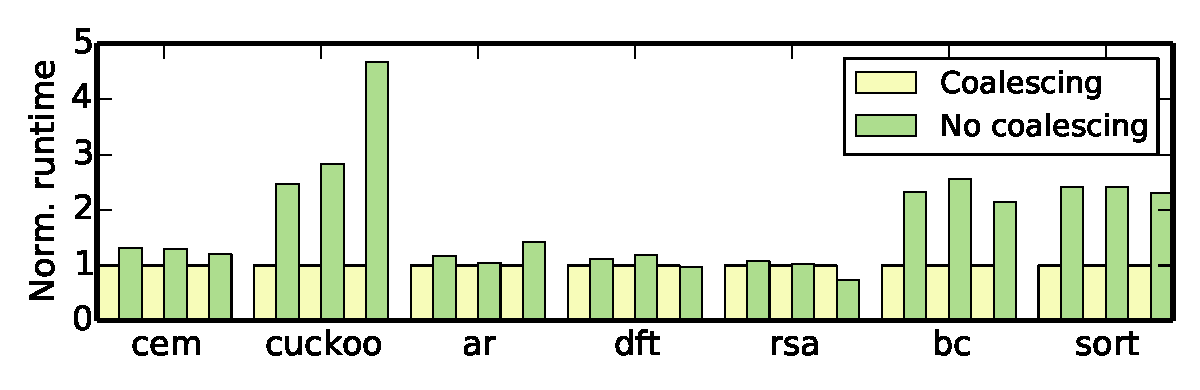
\includegraphics[width=\columnwidth]{figures/coalescing}
	\caption{\sys coalescing performance measured per application at fixed power and various WISP to RFID antenna distances, \{20, 40, 60\}\,cm, assessed against non-coalescing \sys.}
	\label{fig:coalescing}
\end{figure}

We measured \sys coalescing performance. Result is provided in Figure~\ref{fig:coalescing}. Result clearly show that coalescing provides a benefit for all applications, providing even seven times improvement for bc application at 40\,cm. 

\begin{figure}
	\centering
	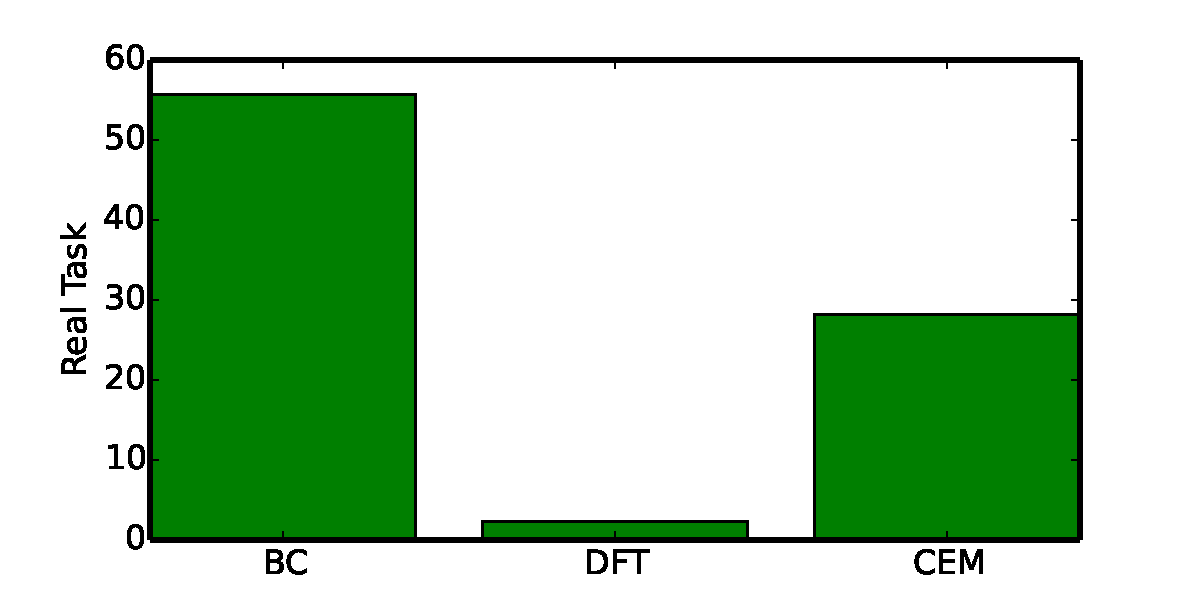
\includegraphics[width=\columnwidth]{figures/averageVirtualTaskSize}
	\caption{Average \sys virtual task size at fixed power per application. Top (green): number of coalesced tasks; bottom (red): average size of real task.}
	\label{fig:aveVirtuTaskSize}
\end{figure}

We need to know how many tasks \sys can coalesce. We ran a subset of applications (split by tasks manually) with continuous power supply and measured the size of tasks for each application and amount of tasks coalesced. Result is given in Figure~\ref{fig:aveVirtuTaskSize}. We see clearly that \sys manages to coalesce more tasks as individual tasks are small. As the size of individual task increases, e.g., as in the case of dft application, the number of coalesced tasks is also small. This result clearly shows that for the benefit of coalescing and for code portability, initial code should be split by \emph{as small tasks as possible}. 

\subsubsection{\sys Paging Performance}
\label{sec:results_memory_management}

\begin{figure}
	\centering
	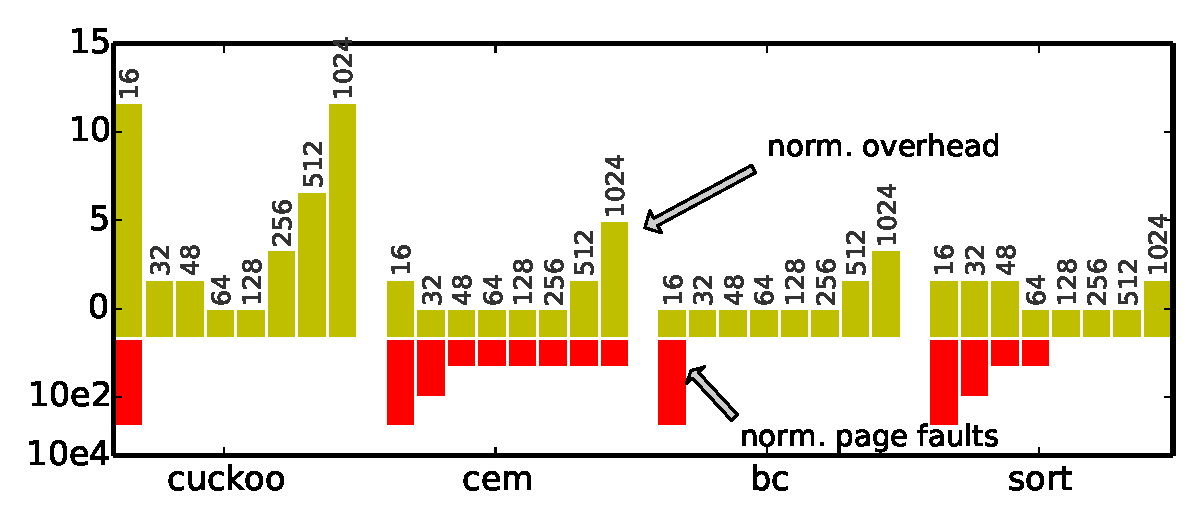
\includegraphics[width=\columnwidth]{figures/pagSizeOverhead}
	\caption{Normalized page size overhead and page faults per benchmark.\todo{Figure placeholder---will be replaced with final one}{Amjad}}
	\label{fig:IPOSPerformance}
	\label{fig:page_size}
\end{figure}

Figure~\ref{fig:page_size} presents the result on the effect of page swap size on the execution time of the programs executed by \sys. Overhead has been measured in the MCU clock cycles with values provided by TI CCS. Result has been normalized per benchmark: for the overhead results---to the minimum obtained value and for page faults---to the third measured maximum value\todo{Check again}{Amjad}. A subset of applications has been selected for evaluation. Additionally, page faults have been measured. The result show clearly a bathtub-shape bar plot for each application, demonstrating that for each application there is always a page size that minimizes \emph{both} execution time and page swaps. For all applications (except for Sort) this value equals roughly to 64 bytes. The shape of each figure can be explained as follows. For small page sizes (<64) the execution time is dominated by the \emph{frequency} of page swaps (each swap takes non-zero time, as shown in Figure~\ref{fig:dmaTimeEnergy}). On the other hand, in the opposite case the execution time is dominated by the time of swapping of one large page from SRAM to FRAM. Another interesting observation is the non-symmetric shape of each bar plot. This is due the size of data manipulated by the program: minimum point of overhead equals roughly to the size of the variables manipulated by each benchmark. Worth noting is also large discrepancy between minimum and maximum overhead for each benchmark (e.g. for Cuckoo 8 (at 16 bytes) to 1 (at 64 bytes), BC: 1 (at 16 bytes) to $\approx$2 (at 1024 bytes)). \todo{Explain this phenomenon}{Amjad}

%\subsubsection{Case Study}
%\label{sec:case_study}

%The final experiment assessing usefulness of \sys's use in real application. For this we have a implemented an battery-less wirelessly-powered sound detector as an example. To the best of our knowledge, this is the first case study that demonstrates a intermittently-powered system supplied by harvested energy at runtime, which continuously interacts with real-life signals. 

%The application aims at detecting a specific tone in the audio signal (in the implementation: 1\,kHz) based on on-the-fly audio measurement. For this we have connected an analog MEMS microphone~\cite{microphone} output to AUX3 port of WISP\,5.1 (while the microphone was powered directly by WISP, which was then wirelessly power-supplied by the RFID reader). Audio signal is sampled by the microcontroller's ADC and passed to the FFT function (internal function of the TI's Digital Signal Processing library~\cite{ti_dsp}) to find a tone above a predefined threshold. The output of the detection is signalled by the WISP on-board LED. The video of demonstrating the working system is available via \url{https://link_to_a_video}.

%Expected results:
%\begin{itemize}
%	\item Compare execution time: \sys against Chain for X\,s long audio signal detection at two antenna distances
%	\item Make a video of the demonstration 
%\end{itemize}
 
%\todo{Check if we really need this application}{Brandon}
%\todo{Provide results and text to this section---if time allows (this result is not critical)}{Amjad/Przemek}
